\documentclass[11pt]{article}
\usepackage[utf8]{inputenc}
\usepackage{amsmath}
\usepackage{amsfonts}
\usepackage{amssymb}

% this is to make it look like a word document.
\usepackage[tmargin=0.98in,bmargin=0.98in,lmargin=1.18in,rmargin=1.18in]{geometry}

% package necessary to add pictures to latex
\usepackage{graphicx}

\usepackage{enumitem}

\title{\vspace{-2ex}Enfoque basado en fronteras para exploración autónoma\vspace{-2ex}}
\date{\today}
\author{Luis Servín\\ Taller TRA, Universidad Nacional Autónoma de México}

\begin{document}

\maketitle

\section*{Resumen}

Se puede definir una \textbf{frontera} en el mapa como el límite entre una región conocida abierta y un espacio aún sin explorar. Basado en esto al moverse a las distintas fronteras dentro de un mapa un robot puede expandir su conocimiento del ambiente que lo rodea. 

El método presentado se basa en los mapas de cuadrícula (\emph{evidence grid}). Una de las principales ventajas que presenta es su capacidad de explorar tanto sitios amplios y abiertos como espacios estrechos desordenados.

\section{Introducción}

Usualmente un mapa para uso humano debe mostrar ya sea la localización exacta de los obstáculos (\emph{mapas métricos}) que existen en el entorno o de una manera gráfica las formas de conexión entre regiones abiertas (\emph{mapas topológicos}). 

Se define el término \textbf{exploración} como la acción de moverse a través de un ambiente desconocido mientras se construye un mapa que puede ser utilizado como base de un sistema de navegación. Por lo tanto una buena estrategia de exploración generará un mapa completo o casi completo de una zona en una cantidad de tiempo razonable.

Aunque durante las simulaciones frecuentemente se ve al mundo como un conjunto de planos. Un robot móvil real tendrá que navegar a través de espacios desordenados, donde las paredes pueden estar escondidas detrás de escritorios o libreros.

Las investigaciones de este tipo aplicadas a ambientes reales han sido escasas. Algunos ejemplos son sistemas de exploración limitados a zonas que pueden ser explorados usando seguimiento de paredes, mientras que otros requieren que dichas paredes se intersecten en ángulos rectos o que dichas paredes no se encuentren obstruidas y sean visibles para el robot.

Dicho lo anterior se busca como objetivo desarrollar una estrategia de exploración basada en fronteras para ambientes complejos como los que se encuentran típicamente en ambientes de oficina.

\section{Exploración Basada en Fronteras}

La pregunta central dentro de la exploración es: Dado lo que conoces acerca del mundo \textbf{¿Hacia que dirección deberías moverte para obtener la mayor cantidad de información posible?} Dado que en un inicio no se tiene conocimiento previo del ambiente mas allá de lo que se puede observar desde el punto en el que te encuentras. Se busca por tanto obtener la mayor cantidad de información como consecuencia de desplazarse hacia una de las fronteras conocidas.

Un robot que cuenta con un mapa perfecto podría navegar a cualquier punto dentro del espacio, dicho punto es considerado \emph{accesible}. Todos lo puntos accesibles tienen la característica de ser continuos ya que debe existir una ruta entre ellos. Si se asumiera que existe un robot cuenta tanto con un sistemas de odometría como sensores perfectos, éste podría aplicar el enfoque de exploración basado en fronteras para explorar la totalidad de su mundo. Pero la pregunta real es ¿Cuál sería su desempeño al trabajar con sistemas que pueden ser afectados por perturbaciones externas en condiciones del mundo real?

\section{Detección de fronteras}

Cada celda dentro del mapa puede ser clasificada si se compara la probabilidad de que se encuentre ocupada contra la probabilidad inicial asignada (generalmente se aplica una probabilidad inicial de 0.5). Dicha clasificación por lo tanto contendría las siguientes categorías:

\begin{itemize}[noitemsep]
	\item \textbf{Abierta o Libre}: $ P_O < P_I $
	\item \textbf{Desconocida}: $ P_O = P_I $
	\item \textbf{Ocupada}: $ P_O > P_I $
\end{itemize}

Donde $ P_O $ es la \textbf{Probabilidad de Ocupación} y $ P_I $ es la \textbf{Probabilidad Inicial}.

\begin{figure}
	\centering
	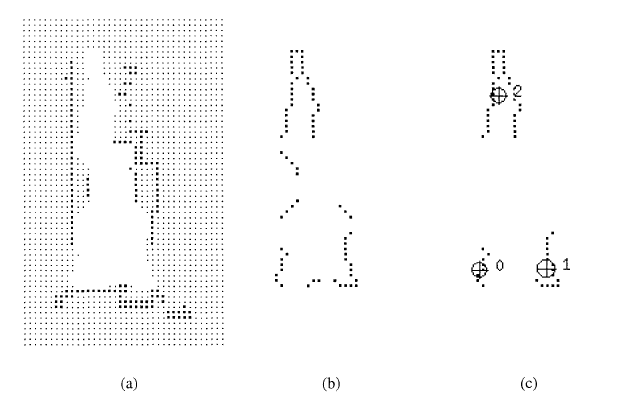
\includegraphics[scale=0.5]{images/frontier_detection.PNG}
	\caption{Detección de la frontera}
	\label{fig:frontier1}
\end{figure}

Cualquier celda libre conocida adyacente a una celda desconocida es etiquetada como una \emph{celda de borde de frontera}. Una serie de celdas de borde de frontera continuas son agrupadas en \emph{regiones de frontera}. Mientras que las regiones de frontera que cumplan con un tamaño mínimo (cercano al tamaño del robot) serán consideradas \textbf{fronteras}.

\section{Navegando hacia las fronteras}

Una vez detectadas las fronteras, el robot intentará navegar hacia la más cercana y accesible que no haya sido visitada aún. Para lograrlo se hace uso de un \emph{algoritmo de planeación de ruta}, para llegar a la ubicación objetivo a través de un camino libre de obstáculos. Durante el recorrido, se hace uso de un comportamiento reactivo de evasión de obstáculos, el cual evita que el robot colisione con algún obstáculo que no fue previsto inicialmente, y regrese a la ruta planeada siempre y cuando no hayan ocurrido cambios muy drásticos en su entorno.

Una vez que el robot ha alcanzado el punto especificado se marca la zona como conocida. Enseguida se realiza un giro de 360 grados ya sea únicamente del sensor o del sistema completo con el objetivo de añadir mas información acerca del entorno, con esta información se actualiza el mapa del entorno.

Este proceso se repite asignando una nueva frontera como objetivo. Si se presenta el caso de que el robot no pueda llegar a su destino después de una cierta cantidad de tiempo, se establece dicho punto como inaccesible y se procede con a alguna otra frontera que aún quede disponible. El algoritmo termina una vez que ya no existe una frontera accesible dentro del mapa sin explorar.

\section{Experimentos}

El experimento descrito dentro del artículo se llevo a cabo utilizando una plataforma \emph{Nomad 200} equipada con un sensor laser, dieciseis sonares, y dieciseis sensores infrarrojos. La totalidad de los sensores infrarrojos y sonares fueron utilizados para la evasión de obstáculos. Se cuenta con un sistema de procesamiento \emph{Sparcstation}. Mientras que la comunicación es realizada por medio de un sistema de radio-ethernet.

Se desarrollaron dos experimentos en ambientes reales de oficina. El primero incluía sillas, escritorios, mesas, libreros, gabinetes, muebles, un enfriador de agua y cajas de distintos tamaños y formas.

En la figura \ref{fig:small_office_map} se muestran los resultados después de un intento.

\begin{figure}[ht]
	\centering
	\begin{minipage}[]{0.45\linewidth}
		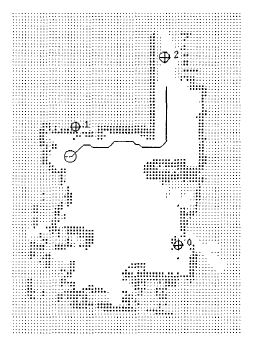
\includegraphics{images/small_office.JPG}
		\caption{Espacio de oficina pequeño}
		\label{fig:small_office_map}
	\end{minipage}
	\quad
	\begin{minipage}[scale=0.]{0.45\linewidth}
		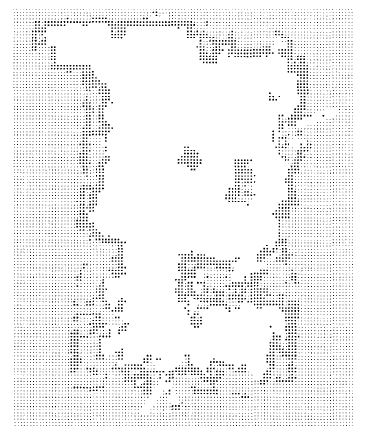
\includegraphics{images/large_office.JPG}
		\caption{Espacio de oficina grande}
		\label{fig:large_office_map}
	\end{minipage}
\end{figure}

Aquellas celdas con baja probabilidad se encontrarse ocupadas son representadas con un espacio en blanco, las que no se conoce su probabilidad con puntos pequeños, mientras que las celdas con altas probabilidades de estar ocupadas con puntos mas grandes. La posición del robot se representa a través de un círculo negro con un línea central que muestra la orientación del robot.

El tiempo total requerido para completar este mapa fue de alrededor de media hora, mientras que una versión mejorada de este algoritmo demostró poder realizar la tarea en alrededor de 15 minutos. El segundo experimento se realizó en un espacio de oficina mucho mas amplio. en la figura \ref{fig:large_office_map} se muestra el mapa obtenido. Aunque el área total fue mayor, el robot fue capaz de completar el espacio en alrededor de media hora. Esto puede deberse a la gran cantidad de espacios libres existentes.

\section*{Conclusiones}

Un robot que hace uso de la exploración basada en fronteras presenta las siguientes ventajas:

\begin{itemize}[noitemsep]
	\item Puede explorar una gran variedad de ambientes, ya sea que tengan amplios espacios abiertos o zonas congestionadas y reducidas.
	\item Las paredes y los obstáculos dentro del espacio a explorar no tienen que cumplir con alguna orientación específica.
	\item La eficiencia aumenta al hacer que el robot se mueva hacia lugares a los cuales tiene mayor probabilidad de obtener nueva información.
\end{itemize}.

% commands for using bibliography and citations 
%\bibliographystyle{ieeetr}
%\bibliography{bibliography}

\end{document}























